% Created 2020-07-19 Sun 22:43
% Intended LaTeX compiler: pdflatex
\documentclass[11pt]{tufte-book}
\usepackage[utf8]{inputenc}
\usepackage[T1]{fontenc}
\usepackage{longtable}
\usepackage{wrapfig}
\usepackage{rotating}
\usepackage[normalem]{ulem}
\usepackage{amsmath}
\usepackage{textcomp}
\usepackage{amssymb}
\usepackage{capt-of}
\usepackage{hyperref}
\usepackage{ucs}
\usepackage{xeCJK}
\setCJKmainfont{STXihei}
\usepackage{graphicx}
  \setkeys{Gin}{width=\linewidth,totalheight=\textheight,keepaspectratio}
  \graphicspath{{graphics/}} % set of paths to search for images
\usepackage{booktabs} % book-quality tables
\usepackage{units}    % non-stacked fractions and better unit spacing
\usepackage{multicol} % multiple column layout facilities
\usepackage{lipsum}   % filler text
\usepackage{fancyvrb} % extended verbatim environments
  \fvset{fontsize=\normalsize}% default font size for fancy-verbatim environments
\setcounter{secnumdepth}{3}
\author{欧阳继超}
\date{\textit{<2017-02-10 Fri>}}
\title{Grokking Monad}
\hypersetup{
 pdfauthor={欧阳继超},
 pdftitle={Grokking Monad},
 pdfkeywords={},
 pdfsubject={},
 pdfcreator={Emacs 26.3 (Org mode 9.1.9)}, 
 pdflang={English}}
\begin{document}

\maketitle
\tableofcontents


\part{第一部分:猫论/Catergory Theory}
\label{sec:org0998dc3}

\begin{center}
\includegraphics[width=.9\linewidth]{./images/Cheshire_Cat.png}
\end{center} \footnote{\url{https://en.wikipedia.org/wiki/Cheshire\_Cat}}

\begin{quote}
`But I don’t want to go among mad people,’ Alice remarked.

`Oh, you can’t help that,’ said the Cat: `we’re all mad here. I’m mad. You’re mad.’

`How do you know I’m mad?’ said Alice.
`You must be,’ said the Cat, `or you wouldn’t have come here.’

Alice didn’t think that proved it at all; however, she went on `And how do you know that you’re mad?’

-- Alice's Adventures in Wonderland
\end{quote}

单子/Monad是什么? 你也不懂, 我也不懂, 我们都不懂.

话说, 我又怎么知道你不懂呢?

当然不懂, 不然, 你怎么会来到这里?

我又是怎么知道自己不懂呢?

因为, 我知道懂的人什么样子. 显然, 我不是.

懂的人一定知道猫论/ Category Theory.

懂猫论的人又不一定知道编程. 但是懂编程的人可以略懂猫论.

编程是项技术, 即理论的降维. 所以要降低门槛, 比如我在书中也\href{https://book.douban.com/subject/26883736/}{写过一章}用JavaScript来解释,某人也尝试过\href{http://www.ruanyifeng.com/blog/2017/02/fp-tutorial.html}{写博客解释},\footnote{如果没看就刚好不要看了, 确实有些误导}没想到那些也不知道会不会 Haskell/Scala 的人就跑出来喷你们前端\footnote{等等, 写前端怎么了? JavaScript 只是我觉得顺手的若干语言之一, JS用户那么多, 写书当然要用 JS 啦, 难道用 Idris 那还能卖得掉吗? \sout{当然最后用JS也没怎么卖掉\ldots{}}}这些不懂函数式的渣渣乱搞出来的东西根本就不是单子。

我也画过一些图来解释,又会被嫌弃画风不好。但是,作为灵魂画师,我只 \sout{是觉得自己萌萌的啊} 在乎画的灵魂是否能够给你一点启发。好吧,讲这么学术的东西,还是用dot来画吧,看起来好正规呢。

好了,安全带系好,我真的要开车了。为了防止解释的不到位/又被喷,就用 Haskell/Scala 好了\footnote{并不是说这两门语言一定在鄙视链顶端, 而是拥有强大类型系统的语言才能体现出范畴论的内容},其实也不难解释清楚 \sout{才怪} 。

这里面很多很装逼的单词,它们都是 \emph{斜体} ,就算没看懂,把这些词背下来也足够装好一阵子逼了/买一阵子萌了。

这里还有很多代码, 它们都成对出现, 第一段是 Haskell, 第二段是 Scala.

\chapter{\emph{Category}}
\label{sec:org7808b7f}
\index{Catergory}
\index{范畴}

一个 \emph{范畴/Category} 包含两个玩意
\begin{itemize}
\item 东西 \texttt{O} (Object)
\item 两个东西的关系,箭头 \texttt{\textasciitilde{}>} ( \emph{态射/Morphism} )
\end{itemize}

还必须带上一些属性: 
\begin{itemize}
\item 一定有一个叫 id 的箭头,也叫做 1
\item 箭头可以 \emph{组合} compose/
\end{itemize}

恩, 就是这么简单!

\begin{figure}[htbp]
\centering
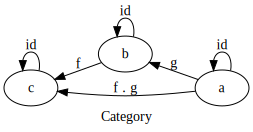
\includegraphics[width=.9\linewidth]{images/category.png}
\caption{有东西 a, b, c 和箭头 f, g 的 Category,其中 f . g 表示 compose f 和 g}
\end{figure}


\begin{quote}
注意到为什么我会箭头从右往左,接着看代码, 你会发现这个方向跟 compose 的方向刚好一致!
\end{quote}

这些玩意对应到 haskell 的 typeclass 大致就是这样:

\begin{verbatim}
class Category (c :: * -> * -> *) where
  id :: c a a
  (.) :: c y z -> c x y -> c x z
\end{verbatim}


而 Scala 可以用 trait 来表示这个 typeclass:
\begin{verbatim}
trait Category[C[_, _]] {
  val id[A]: C[A, A]
  def <<<(a: C[Y, Z], b: C[X, Y]): C[X, Z] 
}
\end{verbatim}

如果这是你第一次见到 Haskell 代码,没有关系,语法真的很简单 \sout{才怪}
\begin{itemize}
\item \texttt{class} 定义了一个 TypeClass, \texttt{Category} 是这个 TypeClass 的名字
\item Type class 类似于定义类型的规范,规范为 \texttt{where} 后面那一坨
\item 类型规范的对象是参数 \texttt{(c:: * -> * -> *)} , \texttt{::} 后面是c的类型
\item c 是 \emph{higher kind} \texttt{* -> *} ,跟higher order function的定义差不多,它是接收类型,构造新类型的类型。这里的 c 接收一个类型,再接收一个类型,就可以返回个类型。
\end{itemize}
\index{Kind}
\begin{itemize}
\item \texttt{id:: c a a} 表示 c 范畴上的 a 到 a 的箭头
\item \texttt{.} 的意思 c 范畴上,如果喂一个 y 到 z 的箭头,再喂一个 x 到 y 的箭头,那么就返回 x 到 z 的箭头。
\end{itemize}

另外 compose 在 haskell 中直接是句号 \texttt{.}

scala 中用 \texttt{<<<} 或者 \texttt{compose}

总之, 用文字再读一遍上面这些代码就了然了.

范畴 C 其实就包含
\begin{enumerate}
\item 返回 A 对象到 A 对象的 id 箭头
\item 可以组合 Y 对象到 Z 对象 和 X 对象到 Y 对象的箭头 compose
\end{enumerate}

简单吧/hen nan ba?还没有高数抽象呢。

\section{\emph{Hask}}
\label{sec:orgac3c44b}
Haskell 类型系统范畴叫做 Hask
\index{Hask}

在 Hask 范畴上:

\begin{itemize}
\item 东西就是类型
\item 箭头是类型的变换,即 \texttt{->}
\item id 就是 id 函数的类型 \texttt{a -> a}
\item compose 当然就是函数组合的类型
\end{itemize}

\begin{verbatim}
type Hask = (->)
instance Category (Hask:: * -> * -> *) where
  (f . g) x = f (g x)
\end{verbatim}

我们看见新的关键字 \texttt{instance} ,这表示 Hask 是 Type class Category 的实例类型,也就是说对任意Hask类型, 那么就能找到它的 id 和 compose

\begin{verbatim}
implicit val haskCat: Category[Hask[_, _]] = new Category[Hask] {
  val id[A] = identity[A]
  def <<<[X, Y, Z](a: Hask[Y, Z], b: Hask[X, Y]) = a compose b
}
\end{verbatim}

Scala 中, 只需要 new 这个 trait 就可以实现这个 typeclass

其中: identity \texttt{Hask a a} 就是
\begin{verbatim}
(->) a a -- or
a -> a -- 因为 -> 是中缀构造器
\end{verbatim}

\begin{verbatim}
A => A
\end{verbatim}
\section{\emph{Duel}}
\label{sec:org510f00a}
\index{Duel}
每个 Category 还有一个镜像,什么都一样,除了箭头是反的

\chapter{函子 / Functor}
\label{sec:orgeff4bd7}
\index{Functor}
\index{函子}
两个范畴中间可以用叫 Functor 的东西来连接起来,简称 T。

\begin{figure}[htbp]
\centering
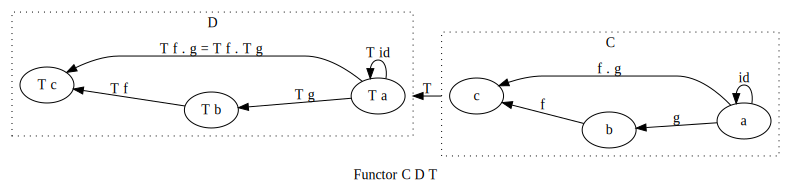
\includegraphics[width=.9\linewidth]{images/functor.png}
\caption{Functor C D T, 从 C 到 D 范畴的Functor T}
\end{figure}

所以大部分把 Functor/Monad 比喻成盒子其实在定义上是错的,虽然这样比喻比较容易理解,在使用上问题也不大。但是,Functor 只是从一个范畴到另一个范畴的映射关系而已。

\begin{itemize}
\item 范畴间 东西的 Functor 标记为 \texttt{T(O)}
\item 范畴间 箭头的 Functor 标记为 \texttt{T(\textasciitilde{}>)}
\item 任何范畴C上存在一个 T 把所有的 O 和 \textasciitilde{}> 都映射到自己,标记为id functor 1\(_{\text{C}}\)
\begin{itemize}
\item 1\(_{\text{C}}\)(O) = O
\item 1\(_{\text{C}}\)(\textasciitilde{}>) = \textasciitilde{}>
\end{itemize}
\end{itemize}

\begin{verbatim}
class (Category c, Category d) => Functor c d t where
  fmap :: c a b -> d (t a) (t b)
\end{verbatim}

\begin{verbatim}
trait Functor[C[_, _], D[_, _], T[_]] {
  def fmap[A, B](c: C[A, B]): D[T[A], T[B]]
}
\end{verbatim}

\texttt{Functor c d t} 这表示从范畴 c 到范畴 d 的一个 Functor t

如果把范畴 c 和 d 都限制到 Hask 范畴

\begin{verbatim}
class Functor (->) (->) t where
  fmap :: (->) a b -> (->) (t a) (t b)
\end{verbatim}

\begin{verbatim}
trait Functor[=>[_, _], =>[_, _], T[_]] {
 def fmap[A, B](c: =>[A, B]): =>[T[A], T[B]]
}
\end{verbatim}
\texttt{->} 在 Haskell 中是中缀类型构造器,所以是可以写在中间的

这样就会变成我们熟悉的 Funtor 的 Typeclass\footnote{这里可以把 Functor 的第一第二个参数消掉, 因为已经知道是在 Hask 范畴了}

\begin{verbatim}
class Functor t where
  fmap :: (a -> b) -> (t a -> t b)
\end{verbatim}

\begin{verbatim}
trait Functor[T[_]] {
 def fmap[A, B](c: A => B): T[A] => T[B]
}
\end{verbatim}

而 \emph{自函子/endofunctor} 就是这种连接相同范畴的 Functor,因为它从范畴 Hask 到达同样的范畴 Hask
\index{endofunctor}
\index{自函子}

这回看代码就很容易对应上图和概念了, 这里的自函子只是映射范畴 \texttt{->} 到 \texttt{->}, 箭头函数那个箭头, 类型却变成了 t a

这里的 fmap 就是 T(\textasciitilde{}>),在 Hask 范畴上,所以是 T(->), 这个箭头是函数,所以也能表示成 T(f) 如果 \texttt{f:: a -> b}

\chapter{\emph{Cat} +猫+/}
\label{sec:org248e5d9}

递归的, 当我们可以把一个 Category 看成一个 object,functor 看成箭头,那么我们又得到了一个 Category,这种 object 是 category 的 category 我们叫它 -- \emph{Cat}

已经没/ meow的办法用语言描述这么高维度的事情了,看图吧\ldots{}

\chapter{自然变换 / Natural Transformations \label{org75e4d4a}}
\label{sec:orgc943a0e}

Functor 是范畴间的映射,所以在这个 Cat 范畴中, 把范畴看成是对象, 那么 Functor 在 Cat 范畴又是个箭头
\index{Natural Transformations}
\index{自然变换}

\begin{center}
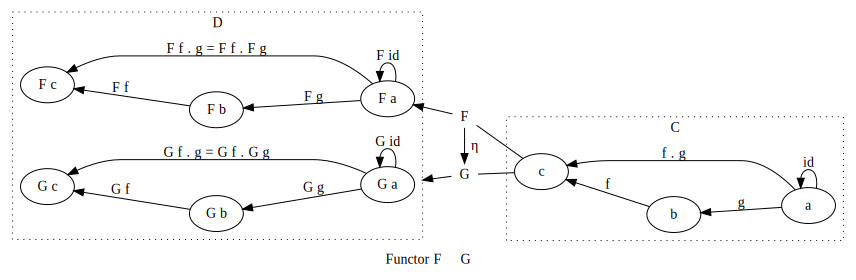
\includegraphics[width=.9\linewidth]{images/natrual-transformation.png}
\end{center}
而 Functor 间也有映射,叫做 \sout{喵的变换} \emph{自然变换}

范畴 c 上的函子 f 到 g 的自然变化就可以表示成
\begin{verbatim}
type Nat c f g = c (f a) (g a)
\end{verbatim}

Scala 没有 rank n type\footnote{别急, 后面马上讲到}, 只能靠 apply 来 meme 了
\begin{verbatim}
trait Nat[C[_, _], F[_], G[_]] {
  def apply[A]: C[F[A], G[A]]
}
\end{verbatim}

Hask 范畴上的自然变化就变成了

\begin{verbatim}
type NatHask f g = f a -> g a
\end{verbatim}

\begin{verbatim}
trait NatHask[F[_], G[_]] {
  def apply[A]: F[A] => G[A]
}

\end{verbatim}

有趣的是, 还可以继续升维度, 比如

\begin{itemize}
\item 东西是函子
\item 箭头是自然变换
\end{itemize}

恭喜你到达 Functor 范畴.

当然, 要成为范畴,还有两个属性:
\begin{itemize}
\item id 为 f a 到 f a 的自然变换
\item 自然变换的组合
\end{itemize}

\begin{center}
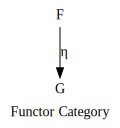
\includegraphics[width=.9\linewidth]{images/functor-category.png}
\end{center}

别着急, 我们来梳理一下,如果已经不知道升了几个维度了,我们假设类型所在范畴是第一维度
\begin{itemize}
\item 一维: Hask, 东西是类型,箭头是 ->
\item 二维: Cat, 东西是 Hask, 箭头是 Functor
\item 三维: Functor范畴, 东西是Functor, 箭头是自然变换
\end{itemize}

感觉到达三维已经是极限了,尼玛还有完没完了,每升一个维度还要起这么多装逼的名字,再升维度老子就画不出来了

所以这时候, 需要引入 String Diagram。

\chapter{String Diagram}
\label{sec:org050993a}

String Diagram 的概念很简单,就是点变线线变点。

还记得当有了自然变换之后,三个维度已经没法表示了,那原来的点和线都升一维度,变成线和面,这样,就腾出一个点来表示自然变换了。

\begin{figure}[htbp]
\centering
\includegraphics[width=.9\linewidth]{images/p1-string-diagram.png}
\caption{String Diagram:自然变换是点,Functor是线,范畴是面}
\end{figure}

compose的方向是从右往左,从下到上。

\chapter{\emph{Adjunction Functor} 伴随函子}
\label{sec:org7e0062a}
\index{Adjunction Functor}
范畴C和D直接有来有回的函子,为什么要介绍这个,因为它直接可以推出 Monad

让我们来看看什么叫有来回。

\begin{center}
\includegraphics[width=.9\linewidth]{images/p1-adjunction-functor.png}
\end{center}

其中:

\begin{itemize}
\item 一个范畴 C 可以通过函子 G 到 D,再通过函子 F 回到 C,那么 F 和 G 就是伴随函子。
\item \(\eta\) 是 GF 到 1\(_{\text{D}}\) 的自然变换
\item \(\epsilon\) 是 1\(_{\text{C}}\) 到 FG 的自然变换
\end{itemize}

同时根据同构的定义,G 与 F 是 \emph{同构} 的。
\index{isomorphic}
\index{同构}

同构指的是若是有
\begin{verbatim}
f :: a -> b
f':: b -> a
\end{verbatim}

那么 f 与 f' 同构,因为 f . f' = id = f' . f

伴随函子的 FG 组合是 C 范畴的 id 函子 F . G = 1\(_{\text{c}}\)

\begin{figure}[htbp]
\centering
\includegraphics[width=.9\linewidth]{images/p1-ajunction-functor-compose.png}
\caption{伴随函子的两个Functor组合, 左侧为 F eta, 右侧为 epsilon F}
\end{figure}

Functor 不仅横着可以组合,竖着(自然变换维度)也是可以组合的,因为自然变换是 Functor 范畴的箭头。

\begin{figure}[htbp]
\centering
\includegraphics[width=.9\linewidth]{images/p1-ajunction-functor-compose-nat.png}
\caption{F eta . epsilon F  = F}
\end{figure}

当到组合 F \(\eta\) . \(\epsilon\) F 得到一个弯弯曲曲的 F 时,我们可以拽着F的两段一拉,就得到了直的 F。

String Diagram 神奇的地方是所有线都可以拉上下两端,这个技巧非常有用,在之后的单子推导还需要用到。

\chapter{从伴随函子到 单子/ Monad}
\label{sec:orgac02402}
有了伴随函子,很容易推出单子,让我们先来看看什么是单子

\begin{itemize}
\item 首先,它是一个 endofunctor T
\item 有一个从 i\(_{\text{c}}\) 到 T 的自然变化 \(\eta\) (eta)
\item 有一个从 T\(^{\text{2}}\) 到 T 的自然变化 \(\mu\) (mu)
\end{itemize}

\begin{center}
\includegraphics[width=.9\linewidth]{images/p1-monad-properties.png}
\end{center}

\begin{verbatim}
class Endofunctor c t => Monad c t where
  eta :: c a (t a)
  mu  :: c (t (t a)) (t a)
\end{verbatim}

\begin{verbatim}
trait Monad[C[_, _], T[_]]] extends Endofunctor[C, T] {
  def eta[A]: C[A, T[A]]
  def mu[A]: C[T[T[A]], T[A]]
}
\end{verbatim}
同样,把 c = Hask 替换进去,就得到更类似我们 Haskell 中 Monad 的定义
\begin{verbatim}
class Endofunctor m => Monad m where
  eta :: a -> (m a)
  mu :: m m a -> m a
\end{verbatim}

\begin{verbatim}
trait Monad[M[_]] extends Endofunctor[M] {
  def eta[A]: A => M[A]
  def mu[A]: M[M[A]] => M[A]
}
\end{verbatim}
要推出单子的 \(\eta\) 变换,只需要让 FG = T
\begin{figure}[htbp]
\centering
\includegraphics[width=.9\linewidth]{images/p1-ajunction-functor-to-monad-eta.png}
\caption{伴随函子的 epsilon 就是单子的 eta}
\end{figure}

同样的,当 FG = T, F \(\eta\) G 就可以变成 \(\mu\)
\begin{figure}[htbp]
\centering
\includegraphics[width=.9\linewidth]{images/p1-ajunction-functor-to-monad-mu.png}
\caption{伴随函子的 F eta G 是函子的 mu}
\end{figure}

\section{三角等式}
\label{sec:org4f1315f}

三角等式是指 \(\mu\) . T \(\eta\) = T = \(\mu\) . \(\eta\) T

要推出三角等式只需要组合 F \(\eta\) G 和 \(\epsilon\) F G
\begin{figure}[htbp]
\centering
\includegraphics[width=.9\linewidth]{images/p1-adjunction-functor-triangle.png}
\caption{F eta G  . epsilon F G = F G}
\end{figure}
\begin{figure}[htbp]
\centering
\includegraphics[width=.9\linewidth]{images/p1-monad-triangle.png}
\caption{F eta G  . epsilon F G= F G 对应到Monad就是 mu . eta T = T}
\end{figure}

换到代码上来说
\begin{verbatim}
(mu . eta) m = m
\end{verbatim}

同样的,左右翻转也成立

\begin{figure}[htbp]
\centering
\includegraphics[width=.9\linewidth]{images/p1-adjunction-functor-triangle-reverse.png}
\caption{F eta G . F G epsilon = F G}
\end{figure}
\begin{figure}[htbp]
\centering
\includegraphics[width=.9\linewidth]{images/p1-monad-triangle-reverse.png}
\caption{F eta G . F G epsilon = F G 对应到 Monad是 mu . T eta = T}
\end{figure}
T \(\eta\) 就是 fmap eta
\begin{verbatim}
(mu . fmap eta) m = m
\end{verbatim}

如果把 \texttt{mu . fmap} 写成 \texttt{>>=} , 就有了

\begin{verbatim}
m >>= eta = m
\end{verbatim}

\section{结合律}
\label{sec:org5e82dc0}

单子另一大定律是结合律,让我们从伴随函子推起

假设我们现在有函子 F \(\eta\) G 和 函子 F \(\eta\) G F G, compose 起来会变成  F \(\eta\) G . F \(\eta\) G F G
\begin{center}
\includegraphics[width=.9\linewidth]{images/p1-ajunction-functor-monad-laws-1.png}
\end{center}

用 F G = T , F \(\eta\) G = \(\mu\) 代换那么就得到了单子的 \(\mu\) . \(\mu\) T
\begin{center}
\includegraphics[width=.9\linewidth]{images/p1-ajunction-functor-monad-laws-2.png}
\end{center}

当组合 F \(\eta\) G 和 F G F \(\mu\) G 后,会得到一个镜像的图
\begin{center}
\includegraphics[width=.9\linewidth]{images/p1-ajunction-functor-monad-laws-3.png}
\end{center}

对应到单子的 \(\mu\) . T \(\mu\)

结合律是说 \(\mu\) . \(\mu\) T = \(\mu\) . T \(\mu\) , 即图左右翻转结果是相等的,为什么呢?看单子的String Diagram 不太好看出来,我们来看伴随函子

如果把左图的左边的 \(\mu\) 往上挪一点,右边的 \(\mu\) 往下挪一点,是不是跟右图就一样了
\begin{center}
\includegraphics[width=.9\linewidth]{images/p1-ajunction-functor-monad-laws-4.png}
\end{center}

结合律反映到代码中就是
\begin{verbatim}
mu . fmap mu = mu . mu
\end{verbatim}

代码很难看出结合在哪里,因为正常的结合律应该是这样的 (1+2)+3 = 1+(2+3),但是不想加法的维度不一样,这里说的是自然变换维度的结合,可以通过String Diagram 很清楚的看见结合的过程,即 \(\mu\) 左边的两个T和先 \(\mu\) 右边两个 T 是相等的。

\chapter{Yoneda lemma / \sout{米田共} 米田引理}
\label{sec:org3127f76}
\index{米田引理}
\index{Yoneda Lemma}

米田引理是说所有Functor \texttt{f a} 一定存在 embed 和 unembed,使得 \texttt{f a} 和 \texttt{(a -> b) -> F b} isomorphic 同构

haskell还要先打开 RankNTypes 的 feature

\begin{verbatim}
{-# LANGUAGE RankNTypes #-}

embed :: Functor f => f a -> (forall b . (a -> b) -> f b)
embed x f = fmap f x

unembed :: Functor f => (forall b . (a -> b) -> f b) -> f a
unembed f = f id
\end{verbatim}

Scala 语言没有 Rank N Type支持, 但是 \hyperref[org75e4d4a]{自然变换/Natural Transformations} 提到过可以用 \texttt{apply} 来模拟. 其实可以使用 Cats 的 \href{https://typelevel.org/cats/datatypes/functionk.html}{FunctionK(\textasciitilde{}>)} 更方便:
\begin{verbatim}
def embed[F[_], A](fa: F[A])(implicit f: Functor[F]): (A => ?) ~> F =
  Lambda[(A => ?) ~> F](f.fmap(_)(fa))
def unembed[F[_]](fnk: (A => ?) ~> F): F[A] =
  fnk(identity)
\end{verbatim}

embed 可以把 functor \texttt{f a} 变成 \texttt{(a -> b) -> f b}

unembed 是反过来, \texttt{(a -> b) -> f b} 变成 \texttt{f a}

上个图就明白了
\begin{figure}[htbp]
\centering
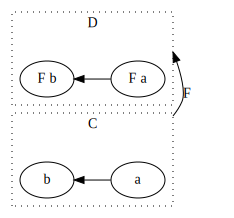
\includegraphics[width=.9\linewidth]{images/yoneda-lemma.png}
\caption{也就是说,图中无论知道a->b 再加上任意一个 F x,都能推出另外一个 F}
\end{figure}

\section{Rank N Type}
\label{sec:orgd750076}
\index{Arbitrary-rank polymorphism}
\index{Rank N Type}

说好的要解释 Rank N Type

Haskell 中可以不用声明类型, 但是其实是省略掉 universally quantified \texttt{forall}, 如果把 forall 全部加回来,
就明了很多:

\begin{itemize}
\item Monomorphic Rank 0 / 0级单态\footnote{也就不是不变态}: t
\item Polymorphic Rank 1 / 1级 \sout{变态} 多态: forall a b. a -> b
\item Polymorphic Rank 2 / 2级多态: forall c. (forall a b. a -> b) -> c
\item Polymorphic Rank 3 / 3级多态: forall d . (forall c . (forall a b . a -> b) -> c) -> d
\end{itemize}

看 rank 几只要数左边 forall 的个数就好了.

一级多态只锁定一次类型 a 和 b

二级多态可以分两次确定类型, 第一次确定 c, 第二次确定 a b

三级多台分三次: 第一次 d, 第二次 c, 第三次 a b

比如:

\begin{verbatim}
rank2 :: forall b c . b -> c -> (forall a. a -> a) -> (b, c)
rank2 b c f = (f b, f c)

rank2 True 'a' id
-- (True, 'a')
\end{verbatim}

\begin{verbatim}
def rank2[B, C](b: B, c: C)(fnk: Id ~> Id): (B, C) =
  (fnk(b), fnk(c))
rank2(true, 'a')(FunctionK.id[Id])
\end{verbatim}

\begin{itemize}
\item f 在 \texttt{f True} 时类型 \texttt{Boolean -> Boolean} 是符合 \texttt{forall a. a->a} 的
\item 与此同时 \texttt{f 'a'} 时类型确实是 \texttt{Char -> Char} 但也符合 \texttt{forall a. a->a}
\end{itemize}

如果是 rank1 类型系统就懵逼了:
\begin{verbatim}
rank1 :: forall a b c . b -> c -> (a -> a) -> (b, c)
rank1 b c f = (f b, f c)
\end{verbatim}

\begin{verbatim}
def rank1[A, B, C](b: B, c: C)(fn: A => A): (B, C) =
  (fn(b), fn(c))
\end{verbatim}
f 在 \texttt{f True} 是确定 a 是 Boolean,在rank1多态是时就确定了 \texttt{a->a} 的类型一定是 \texttt{Boolean -> Boolean}

所以到 \texttt{f 'a'} 类型就挂了。

\chapter{\emph{Kleisli Catergory}}
\label{sec:orgab35996}
\index{Kleisi Catergory}

\begin{figure}[htbp]
\centering
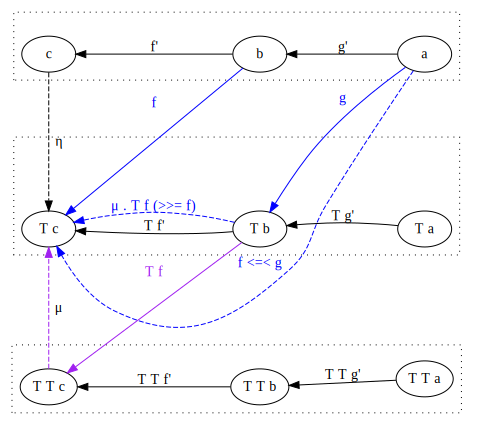
\includegraphics[width=.9\linewidth]{images/kleisli.png}
\caption{注意观察大火箭 <=< 的轨迹, 不知道dot为什么会把这根线搞这么又弯又骚的, 和 >>= 。所以 Kleisli 其实就是斜着走的一个范畴,但是 >>= 把它硬生生掰 \sout{弯} 直了。}
\end{figure}

函子/Functor 的范畴叫做 函子范畴/Functor Catergory, 自然变换是其箭头。那单子/Monad也可以定义一个范畴吗?\footnote{当然, 单子是自函子,所以也可以是自函子范畴}

是的, 这个范畴名字叫做 \sout{单子范畴}\footnote{怎么说也是函数式编程的核心,怎么可以叫的这么low这么直接} 可莱斯利范畴/Kleisli Catergory\footnote{这个是我瞎翻译的, 但是读出来就是这么个意思, 真的, 不骗你, 照这么读绝对装的一手好逼, 不会被嘲笑的},那么 Kleisli 的箭头是什么?
我们看定义,Kleisli Catergory

\begin{enumerate}
\item 箭头是 Kleisli 箭头 \texttt{a -> T b}
\item 东西就是c范畴中的东西. 因为 a 和 b 都是 c 范畴上的, 由于T是自函子,所以 T b 也是 c 范畴的
\end{enumerate}

看到图上的 T f/ fmap f 和 \(\mu\) 了没?\footnote{(敲黑板) 就是紫色那根嘛!}

\begin{verbatim}
f :: b -> T c
fmap f :: T b -> T T c
mu :: T T c -> T c
\end{verbatim}

\begin{verbatim}
def f[T[_], B, C](b: B): T[C]
def fmap[T[_], B, C](f: B => C)(tb: T[B]): T[T[C]]
def mu[T[_], C](ttc: T[T[C]]): T[C]
\end{verbatim}

紫色的箭头 \texttt{T f}\footnote{即 \texttt{fmap f}} 和紫色的虚线箭头 \(\mu\) 连起来就是 \texttt{T f'}, 那么最出名的 \texttt{>>=} 符号终于出来了:
\begin{verbatim}
tb >>= f = (mu . fmap f) tb
\end{verbatim}

\begin{verbatim}
def flatMap[T[_], B, C](f: B => T[C])(tb: T[B]): T[C] = (mu compose fmap(f))(tb)
\end{verbatim}

下面这个大火箭 \texttt{<=<} 可以把蓝色箭头组合起来.
\begin{verbatim}
(f <=< g) = mu . T f . g = mu . fmap f . g
\end{verbatim}

\begin{verbatim}
def <=<[T[_], A, B, C](f: B => T[C])(g: A => T[B]): A => T[C] =
  mu compose fmap(f) compose g
\end{verbatim}

因此大火箭就是 Kleisli 范畴的 \texttt{compose}

\begin{verbatim}
(<=<) :: Monad T => (b -> T c) -> (a -> T b) -> (a -> T c)
\end{verbatim}

\chapter{Summary}
\label{sec:org493098f}
第一部分理论部分都讲完了, 如果你读到这里还没有被这些吊炸天/乱七八糟的概念搞daze,接下来可以看看它到底跟我们编程有鸟关系呢?第二部分将介绍这些概念产生的一些实用的monad

\begin{itemize}
\item 👉 \href{./part2.org}{第二部分:食用猫呢/ Practical Monads}
\item \href{./part3.org}{第三部分:搞基猫呢/ Advanced Monads}
\end{itemize}

当然我还没空全部写完,如果有很多人预定/只要998 Gumroad 上的  电子书的话,我可能会稍微写得快一些。毕竟,写了也没人感兴趣也怪浪费时间的。不过,我猜也没几个人能看到这一行,就当是自言自语吧,怎么突然觉得自己好分裂。

\part{第二部分:食用猫呢/ Practical Monads}
\label{sec:org79df89b}

\begin{center}
\includegraphics[width=.9\linewidth]{./images/Alice_through_the_looking_glass.jpg}
\end{center}

\begin{quote}
“If I had a world of my own, everything would be nonsense. 
Nothing would be what it is, because everything would be what it isn't.
And contrary wise, what is, it wouldn't be. And what it wouldn't be, it would. You see?”
― Lewis Carroll, Alice's Adventures in Wonderland \& Through the Looking-Glass 
\end{quote}

如果有一个单子的世界, 那一切都说不通了.
没有什么是应该的, 因为所有东西都是它不是的东西.
反过来说, 是又不会是, 而不会是的又会是. 懂没?

到底什么是, 什么不是, 我们看编程世界里到底什么是单子?

这一部分将介绍由一些实用的单子实例/monad instances,通过这些单子实例,解决了分离计算与副作用, 已经组合性的问题。

\chapter{Identity 本身就有}
\label{sec:orgf411766}

本身就有单子/ Identity Monad\footnote{从来没见过有人给这些数据类型按过中文名字, 不然我来, 这样也更好的体会这些数据类型的意图.} 可能是最简单的单子了。本身不包含任何计算, 且只有一个构造器:
\begin{verbatim}
newtype Identity a = Identity { runIdentity :: a }
\end{verbatim}

\begin{verbatim}
case class Identity[A](run: A)
\end{verbatim}

这里使用 \texttt{newtype} 而不是 \texttt{data} 是因为 \texttt{Identity} 与 \texttt{runIdentity} 是同构的\footnote{见 \href{part1.org}{第一部分 伴随函子}}.

\begin{verbatim}
Identity :: a -> Identity a
runIdentity :: Identity a -> a
\end{verbatim}

你看 \texttt{runIdentity . Identity = id} ,所以他们是同构的。

左边的 \texttt{Identity} 是类型构造器\footnote{也就是 Kind * -> *, 因为它非常的 nice, 一定要等到 a 才出类型}, 接收类型 \texttt{a} 返回 \texttt{Identity a} 类型

如果 a 是 Int,那么就得到一个 \texttt{Identity Int} 类型。

右边的 \texttt{Identity} 是数据构造器,也就是构造值,比如 \texttt{Identity 1} 会构造出一个值,其类型为 \texttt{Identity Int}

大括号比较诡异,可以想象成给 \texttt{a} 一个 key,同过这个 key 可以把 a 取出来,比如
\begin{verbatim}
runIdentity (Identity 1)
\end{verbatim}

\begin{verbatim}
Identity(1).run
\end{verbatim}

会返回 1

Identity 可以实现 Functor 和 Monad,就得到 Identity functor 和 Identity monad:

\begin{verbatim}
instance Functor Identity where
  fmap f (Identity a) = Identity (f a)

instance Monad Identity where
  return a = Identity a
  Identity a >>= f = f a
\end{verbatim}

而 Scala 则需要用 \texttt{implicit} 来实现 typeclass:

\begin{verbatim}
implicit val identityFunctor: Functor[Identity] = new Functor[Identity] {
  def fmap[A, B](f: A => B): Identity[A] => Identity[B] = {
    case Identity(a) => Identity(f(a))
  }
}

implicit val identityMonad: Monad[Identity] = new Monad[Identity] {
  def pure[A](a: A): Id[A] = Identity(a)
  def flatMap[A, B](f: A => Identity[B]): Identity[A] => Identity[B] = {
    case Identity(a) => f(a)
  }
}
\end{verbatim}

可以看到 Identity 即是构造器/constructor,也是解构器/destructure,利用模式匹配是可以解构出值的。

例如上面 Functor 实现中的 \texttt{fmap f (Identity a)}, 假如 \texttt{fmap} 的是 \texttt{Identity 1},
那么这个模式匹配到 \texttt{(Identity a)} 时会通过解构器把 \texttt{1} 放到 \texttt{a} 的位置。

Identity 看起来什么也没有干,就跟 identity 函数一样,但是实际上, 它也跟 identity 相对于函数一样
相对于类型非常有用.

\chapter{Maybe 可能会有}
\label{sec:orgb9eb3c2}
可能会有单子/Maybe Monad是一个超级简单的但比本身就有稍稍复杂的单子.

因为它拥有比本身就有多一个的类型构造器,类似这样的叫做 代数数据类型/ Algebra Data Type(ADT)

\begin{verbatim}
data Maybe a = Just a | Nothing
\end{verbatim}

你看, 不管是 \texttt{Just} 还是 \texttt{Nothing} 都可以构造出一个 \texttt{Maybe} 类型的数据来.

ADT 在 Scala 可以用 trait 表示, 而且, Scala 中的 \texttt{Maybe} 叫做 \texttt{Option}:

\begin{verbatim}
trait Option[+A]
case class Some[A](a: A) extends Option[A]
case object None extends Option[Nothing]
\end{verbatim}

Haskell 中定义一个 ADT 十分简单,不像 Scala 那么啰嗦。左边是类型构造器,右边有数据构造器,你会发现有一根竖线 \texttt{|} , 它分隔着两个构造器
\begin{itemize}
\item \texttt{Just}
\item \texttt{Nothing}
\end{itemize}

其中 \texttt{a} \footnote{一定要记得小写哦}表示是任意类型.

所以 \texttt{Just 1} 会得到一个 \texttt{Num a => Mabye a} 类型\footnote{意思就是 \texttt{Maybe a} 但是 \texttt{a} 的类型约束为 \texttt{Num}},
\texttt{Nothing} 也会得到一个 \texttt{Maybe a} 只不过 \texttt{a} 没有类型约束。

总之我们有了构造器可以构造出 \texttt{Maybe} 类型,而这个类型能做的事情,就要取决它实现了哪些 typeclass 的 instance 了。比如它可以是一个函子.
\begin{verbatim}
instance Functor Maybe where
  fmap f (Just a) = Just (f a)
  fmap f Nothing = Nothing
\end{verbatim}

\begin{verbatim}
implicit val optionFunctor: Functor[Option] = new Functor[Option] {
  def fmap[A, B](f: A => B): Option[A] => Option[B] = {
    case Some(a) => Some(f(a))
    case None => None
  }
}
\end{verbatim}

\begin{figure}[htbp]
\centering
\includegraphics[width=.9\linewidth]{images/p2-maybe-functor.png}
\caption{fmap :: (a -> b) -> f a -> f b}
\end{figure}

看清楚了, 虚线箭头即 \texttt{fmap}, 图上表示的 \texttt{fmap} 是 \texttt{(a -> b) - - -> (Maybe a -> Maybe b)} 由于这里的箭头都是在 \texttt{->} 范畴, 所以 \texttt{- - ->} 就是 \texttt{->} 了.

即: \texttt{fmap :: (a -> b) -> f a -> f b}

不仅如此,还可以实现单子:
\begin{verbatim}
instance Monad Maybe where
  return a = Just a
  (Just a) >>= f = f a
  Nothing >>= f = Nothing
\end{verbatim}

\begin{verbatim}
implicit val optionMonad: Monad[Option] = new Monad[Option] {
  def flatMap[A, B](f: A => Option[B]): Option[A] => Option[B] = {
    case Some(a) => f(a)
    case None => None
  }
}
\end{verbatim}

\begin{figure}[htbp]
\centering
\includegraphics[width=.9\linewidth]{images/p2-maybe-kleisli.png}
\caption{还记得第一部分提到的 Kleisli 范畴吗?}
\end{figure}

Maybe 有用在于能合适的处理 \emph{偏函数} Partial Function/ 的返回值。
偏函数相对于 \emph{全函数} Total Function/ 是指只能对部分输入返回输出的函数。

比如一个取数组某一位上的值的函数,就是偏函数,因为假设你想取第4位的值,但不是所有数组长度都大于4,就会有获取不了的尴尬情况。
\begin{verbatim}
[1,2,3] !! 4
\end{verbatim}

\begin{verbatim}
List(1,2,3).get(4)
\end{verbatim}

如果使用 Maybe 把偏函数处理不了的输入都返回成 Nothing,这样结果依然保持 Maybe 类型,不影响后面的计算。

\chapter{Either 要么有要么有}
\label{sec:orgdb30dec}

Either 的定义也很简单
\begin{verbatim}
data Either a b = Left a | Right b
\end{verbatim}

\begin{verbatim}
trait Either[+A, +B]
case class Left[+A, +B](a: A) extends Either[A, B]
case class Right[+A, +B](b: B) extends Either[A, B]
\end{verbatim}


\section{Product \& Coproduct}
\label{sec:org94ad970}
看过第一部分应该还能记得有一个东西叫 Duel,所以见到如果范畴上有 Coproduct 那么肯定在duel范畴上会有同样的东西叫 Product。

那么我们先来看看什么是 Coproduct

\begin{figure}[htbp]
\centering
\includegraphics[width=.9\linewidth]{images/p2-coproduct.png}
\caption{Coproduct}
\end{figure}

像这样,能通过两个箭头到达同一个东西,就是 Coproduct。这里箭头 \texttt{Left} 能让 \texttt{a} 到 \texttt{Either a b} , 箭头 \texttt{Right} 也能让 \texttt{b} 到达 \texttt{Either a b}

有意思的是还肯定存在一个 Coproduct 和 箭头,使得下图成立
\begin{center}
\includegraphics[width=.9\linewidth]{images/p2-coproduct-law.png}
\end{center}

箭头反过来,就是 Product, 比如 Tuple

\begin{figure}[htbp]
\centering
\includegraphics[width=.9\linewidth]{images/p2-product.png}
\caption{Product}
\end{figure}

Tuple 的 \texttt{fst} 箭头能让 \texttt{(a, b)} 到达 \texttt{a} 对象,而箭头 \texttt{snd} 能让其到达 \texttt{b} 对象。

\section{Either Monad}
\label{sec:orgd190698}
确切的说,Either 不是 monad, \texttt{Either a} 才是。还记得 monad 的 class 定义吗?
\begin{verbatim}
class Endofunctor m => Monad m where
  eta :: a -> (m a)
  mu :: m m a -> m a
\end{verbatim}
所以 m 必须是个 Endofunctor,也就是要满足 Functor
\begin{verbatim}
class Functor t where
  fmap :: (a -> b) -> (t a -> t b)
\end{verbatim}
t a 的 kind 是 *,所以 t 必须是 kind * -> *
也就是说,m 必须是接收一个类型参数的类型构造器

而 Either 的 kind 是 * -> * -> *, Either a 才是 * -> *

所以只能定义 Either a 的 Monad
\begin{verbatim}
instance Monad (Either a) where
  Left  l >>= _ = Left l
  Right r >>= k = k r
\end{verbatim}

很明显的,>>= 任何函数到左边/ Left 都不会改变,只有 >>= 右边才能产生新的计算。


\chapter{Reader 差一点就有}
\label{sec:org7a33c1e}
Reader 的作用是给一个计算喂数据。

在描述计算的时候,并不需要关心输入时什么,只需要 asks 就可以拿到输入值

而真正的输入,会在运行计算时给予。

跟 Identity 一样,我们用 newtype 来定义一个同构的 Reader 类型
\begin{verbatim}
newtype Reader e a = Reader { runReader :: (e -> a) }
\end{verbatim}

其中
\begin{itemize}
\item e 是输入
\item a 是结果
\item 构造 Reader 类型需要确定 输入的类型 e 与输出的类型 a
\item \texttt{runReader} 的类型是 \texttt{runReader:: (Reader e a) -> (e -> a)}
\end{itemize}

也就是说在描述完一个 Reader 的计算后,使用 runReader 可以得到一个 e -> a 的函数,使用这个函数,就可以接收输入,通过构造好的计算,算出结果 a 返回。

那么,让我们来实现 Reader 的 monad instance,就可以描述一个可以 ask 的计算了。

\begin{verbatim}
instance Monad (Reader e) where
    return a         = Reader $ \_ -> a
    (Reader g) >>= f = Reader $ \e -> runReader (f (g e)) e
\end{verbatim}

跟Either一样,我们只能定义 Reader e 的 monad instance。

注意这里的
\begin{itemize}
\item f 类型是 \texttt{(a -> Reader e a)}
\item g 其实就是是 destructure 出来的 runReader,也就是 e -> a
\item 所以 (g e) 返回 a
\item f (g e) 就是 \texttt{Reader e a}
\item 再 run 一把最后得到 a
\end{itemize}

\begin{figure}[htbp]
\centering
\includegraphics[width=.9\linewidth]{images/p2-reader-monad.png}
\caption{f 函数,接收 a 返回一个 从 e 到 a 的 Reader}
\end{figure}

让我们来看看如何使用 Reader
\begin{verbatim}
import Control.Monad.Reader

data Environment = Env
  { fistName :: String
  , lastName :: String
  } deriving (Show)

helloworld :: Reader Environment String
helloworld = do
  f <- asks firstName
  l <- asks lastName
  return "Hello " ++ f ++ l

runHelloworld :: String
runHelloworld = runReader helloworld $ Env "Jichao" "Ouyang"
\end{verbatim}

这段代码很简单,helloworld 负责打招呼,也就是在名字前面加个 "Hello",而跟谁打招呼,这个函数并不关心,而单纯的是向 Environment 问/asks 就好。

\begin{figure}[htbp]
\centering
\includegraphics[width=.9\linewidth]{images/p2-reader-monad-ask.png}
\caption{asks 可以将 e -> a 的函数变换成 Reader e a}
\end{figure}

在运行时,可以提供给 Reader 的输入 Env fistname lastname。
\begin{center}
\includegraphics[width=.9\linewidth]{images/p2-reader-monad-run.png}
\end{center}

\section{do notation}
\label{sec:orgc161d0d}
这可能是你第一次见到 \texttt{do} 和 \texttt{<-}. 如果不是,随意跳过这节。

\begin{itemize}
\item do 中所有 <- 的右边都是 \texttt{Reader Environment String} 类型
\item do 中的 return 返回类型也必须为  \texttt{Reader Environment String}
\item \texttt{asks firstName} 返回的是 \texttt{Reader Environment String} 类型, \texttt{<-} 可以理解成吧 monad \texttt{Reader Environment} 的内容放到左边的 f, 所以 f 的类型是 String。
\end{itemize}

看起来像命令式的语句,其实只是 \texttt{>>=} 的语法糖,但是明显用do可读性要高很多。
\begin{verbatim}
helloworld = (asks firstName) >>=
  \f -> (asks lastName) >>=
       \l -> return "Hello " ++ f ++ l
\end{verbatim}


\chapter{Writer 光出进没有}
\label{sec:orgfc9110a}

除了返回值,计算会需要产生一些额外的数据,比如 log

此时就需要一个 Writter,其返回值会是一个这样 \texttt{(result, log)} 的 tuple

限制是 log 的类型必须是个 含幺半群/monoid

\begin{verbatim}
example :: Writer String String
example  = do
  tell "How are you?"
  tell "I'm fine thank you, and you?"
  return "Hehe Da~"

output :: (String, String)
output = runWriter example
-- ("Hehe Da~", "How are you?I'm fine thank you, and you?")
\end{verbatim}

Writer 的定义更简单
\begin{verbatim}
newtype Writer l a = Writer { runWriter :: (a,l) }
\end{verbatim}
里面只是一个 tuple 而已
\begin{itemize}
\item w 是 log
\item a 是 返回值
\end{itemize}

看看如何实现 Writer monad
\begin{verbatim}
instance (Monoid w) => Monad (Writer w) where
    return a             = Writer (a,mempty)
    (Writer (a,l)) >>= f = let (a',l') = runWriter $ f a in
                           Writer (a',l `mappend` l')
\end{verbatim}

\begin{itemize}
\item return 不会有任何 log,l 是 monoid 的 mempty
\item f 的类型为 \texttt{a -> Writer l a}
\item \texttt{runWriter \$ f a} 返回 \texttt{(a, l)}
\end{itemize}

\begin{center}
\includegraphics[width=.9\linewidth]{images/p2-writer-monad.png}
\end{center}

所以在 >>= 时,我们先把 f a 返回的 Writer run了,然后把两次 log \texttt{mappend} 起来。
\begin{center}
\includegraphics[width=.9\linewidth]{images/p2-writer-monad-bind.png}
\end{center}

\chapter{State 变化会有}
\label{sec:orgf83aa9d}
跟名字就看得出来 State monad 是为了处理状态。虽然函数式编程不应该有状态,不然会引用透明性。但是,state monad并不是在计算过程中修改状态,而是通过描述这种变化,然后需要时在运行返回最终结果。这一点跟 Reader 和 Writer 这两个看起来是副作用的 IO 是一样的。

先看下 State 类型的定义
\begin{verbatim}
newtype State s a = State { runState :: s -> (a, s) }
\end{verbatim}

可以看到 State 只包含一个 从旧状态 s 到新状态 s 和返回值 a 的 Tuple 的函数。

通过实现 Monad,State 就可以实现命令式编程中的变量的功能。
\begin{verbatim}
instance Monad (State s) where
  return a        = State $ \s -> (a,s)
  (State x) >>= f = State $ \s -> let (v,s') = x s in
                                 runState (f v) s'
\end{verbatim}
return 很简单,就不用解释了。

\begin{center}
\includegraphics[width=.9\linewidth]{images/p2-state-monad.png}
\end{center}

x 类型是 \texttt{s -> (a, s)} ,所以 x s 之后会返回 结果和状态。也就是运行当前 State,把结果 v 传给函数 f,返回的 State 再接着上次状态运行。

\begin{figure}[htbp]
\centering
\includegraphics[width=.9\linewidth]{images/p2-state-monad-bind.png}
\caption{State x >>= f 后runState的数据流(啊啊啊,画歪了,感觉需要脉动一下)}
\end{figure}

使用起来也很方便,State 提供 \texttt{get} \texttt{put} \texttt{moidfy} 三个方便的函数可以生成修改状态的State monad

\begin{verbatim}
import Control.Monad.Trans.State.Strict
test :: State Int Int
test = do
  a <- get
  modify (+1)
  b <- get
  return (a + b)

main = print $ show $ runState test 3
-- (7, 4)
\end{verbatim}


\chapter{Validation 检查检查}
\label{sec:org7d09bfd}
如果你有注意到,前面的 Either 可以用在处理错误和正确的路径分支,但是问题是错误只发生一次。

\begin{quote}
Validation 没有在标准库中,但是我觉得好有用啊,你可以在 ekmett 的 \href{https://github.com/ekmett/either}{github} 中找到源码
\end{quote}

想象一下这种场景,用户提交一个表单,我们需要对每一个field进行验证,如果有错误,需要把错误的哪几个field的错误消息返回。显然如果使用 Either 来做,只能返回第一个field的错误信息,后面的计算都会被跳过。

针对这种情况, Validation 更适合
\begin{verbatim}
data Validation e a = Failure e | Success a
\end{verbatim}

ADT定义看起来跟 Either 是一样的,不同的是 左边/Left Failure 是 含幺半群/Monoid

\section{含幺半群/Monoid}
\label{sec:orga56ba93}
monoid 首先得是 半群/Semigroup ,然后再 含幺。
\begin{verbatim}
class Semigroup a where
  (<>) :: a -> a -> a
  (<>) = mappend
\end{verbatim}

半群非常简单,只要是可以 \texttt{<>} (mappend) 的类型就是了。

含幺只需要有一个 \texttt{mempty} 的 幺元就行
\begin{verbatim}
class Monoid a where
  mempty  :: a
  mappend :: a -> a -> a
\end{verbatim}

比如 List 就是 Semigroup
\begin{verbatim}
instance Semigroup [a] where
  (<>) = (++)
\end{verbatim}
也是 Monoid
\begin{verbatim}
instance Monoid [a] where
  mempty  = []
  mappend = (++)
\end{verbatim}

Monoid 的 \texttt{<>} 满足:
\begin{itemize}
\item mempty <> a = a
\item a <> b <> c = a <> (b <> c)
\end{itemize}
\section{回到 Validation}
\label{sec:org653eaa8}
现在让 Failure e 满足 Monoid,就可以 \texttt{mappend} 错误信息了。
\begin{verbatim}
instance Semigroup e => Semigroup (Validation e a) where
  Failure e1 <> Failure e2 = Failure (e1 <> e2)
  Failure _  <> Success a2 = Success a2
  Success a1 <> Failure _  = Success a1
  Success a1 <> Success _  = Success a1
\end{verbatim}

下来,我们用一个简单的例子来看看 Validation 与 Either 有什么区别。

假设我们有一个form,需要输入姓名与电话,验证需要姓名是非空而电话是11位数字。

首先,我们需要有一个函数去创建包含姓名和电话的model
\begin{verbatim}
data Info = Info {name: String, phone: String} deriving Show
\end{verbatim}

然后我们需要验证函数
\begin{verbatim}
notEmpty :: String -> String -> Validation [String] String
notEmpty desc "" = Failure [desc <> " cannot be empty!"]
notEmpty _ field = Success field
\end{verbatim}
notEmpty 检查字符是否为空,如果是空返回 Failure 包含错误信息,若是非空则返回 Success 包含 field

同样的可以创建 11位数字的验证函数
\begin{verbatim}
phoneNumberLength :: String -> String -> Validation [String] String
phoneNumberLength desc field | (length field) == 11 = Success field
                             | otherwise = Failure [desc <> "'s length is not 11"]
\end{verbatim}
实现 Validation 的 Applicative instance,这样就可以把函数调用lift成带有验证的 Applicative
\begin{verbatim}
instance Semigroup e => Applicative (Validation e) where
  pure = Success
  Failure e1 <*> Failure e2 = Failure e1 <> Failure e2
  Failure e1 <*> Success _  = Failure e1
  Success _  <*> Failure e2 = Failure e2
  Success f <*> Success a = Success (f a)
\end{verbatim}
\begin{itemize}
\item 失败应用到失败会 concat 起来
\item 失败跟应用或被成功应用还是失败
\item 只有成功应用到成功才能成功,这很符合验证的逻辑,一旦验证中发生任何错误,都应该返回失败。
\end{itemize}

\begin{verbatim}
createInfo :: String -> String -> Validation [String] Info
createInfo name phone = Info <$> notEmpty "name" name <*> phoneNumberLength "phone" phone
\end{verbatim}

现在我们就可以使用带validation的 createInfo 来安全的创建 Info 了

\begin{verbatim}
createInfo "jichao" "12345678910" -- Success Info "jichao" "12345678910"
createInfo "" "123" -- Failure ["name cannot be empty!", "phone's length is not 11"]
\end{verbatim}

\chapter{Cont 接下来有}
\label{sec:org11a1a3d}
Cont 是 Continuation Passing Style/CPS 的 monad,也就是说,它是包含 cps 计算 monad。

先看一下什么是 CPS,比如有一个加法
\begin{verbatim}
add :: Int -> Int -> Int
add = (+)
\end{verbatim}

但是如果你想在算法加法后,能够继续进行一个其他的计算,那么就可以写一个 cps版本的加法
\begin{verbatim}
addCPS :: Int -> Int -> (Int -> r) -> r
addCPS a b k = k (a + b)
\end{verbatim}

非常简单,现在我们可以看看为什么需要一个 Cont monad 来包住 CPS 计算,首先,来看 ADT 定义
\begin{verbatim}
newtype Cont r a = Cont { runCont :: ((a -> r) -> r) }
\end{verbatim}

又是一个同构的类型,Cont 构造器只需要一个 runCount,也就是让他能继续计算的一个函数。

完了之后来把之前的 addCPS 改成 Cont
\begin{verbatim}
add :: Int -> Int -> Cont k Int
add a b = return (a + b)
\end{verbatim}

注意到 addCPS 接收到 a 和 b 之后返回的类型是 \texttt{(Int -> r) -> r} ,而 Cont 版本的 \texttt{add} 返回 \texttt{Cont k Int}

明显构造 \texttt{Cont k Int} 也正是需要 \texttt{(Int -> r) -> r} ,所以 Cont 就是算了 k 的抽象了。

\begin{verbatim}
instance Monad (Cont r) where
    return a = Cont ($ a)
    m >>= k  = Cont $ \c -> runCont m $ \a -> runCont (k a) c
\end{verbatim}

\texttt{(\$ a)} 比较有意思, 我们都知道 \texttt{f \$ g a} 其实就是 \texttt{f(g a)}, 所以 \texttt{\$} 其实就是一个 apply 左边的函数到右边表达式的中缀函数, 如果写成前缀则是
\texttt{(\$ (g a) f)}. 是反的是因为 \texttt{\$} 是有结合, 需要右边表达式先求值, 所以只给一个 a 就相当于 \texttt{(\$ a) = \textbackslash{}f -> f a}

回到 Monad Cont\ldots{}

\chapter{Summary}
\label{sec:orgd1fdd56}
第二部分食用部分也讲完了, 不知是否以及大致了解了monad的尿性各种基本玩法呢?通过这些常用的基本的 monad instance,解决命令式编程中的一些简单问题应该是够了。

不过,接下来还有更变态的猫,就先叫她 \sout{搞基} 猫呢好了。

\begin{itemize}
\item 👉 \href{./part3.org}{第三部分:搞基猫呢/ Advanced Monads}
\end{itemize}

当然我又还没空全部写完,如果还有很多人预定/只要998 Gumroad 上的  电子书的话,我可能会稍微写得快一些。毕竟,写了也没人感兴趣也怪浪费时间的。不过,我猜也没几个人能看到这一行,就当是我又自言自语吧,怎么又突然觉得自己好分裂,诶\textasciitilde{},为什么我要说又?

\part{第三部分:搞基猫呢/Advanced Monads}
\label{sec:org55db55f}
第二部分介绍了一些实用的monad instances,这些 monad 都通过同样的抽象方式,解决了分离计算与副作用的工作。

通过它们可以解决大多数的基本问题,但是正对于复杂业务逻辑,我们可能还需要一些更高阶的 monad 或者 pattern。

当有了第一部分的理论基础和第二部分的实践,这部分要介绍的猫呢其实并不是很搞基。通过这一部分介绍的搞基猫呢,
我们还可以像 IO monad 一样,通过 free 或者 Eff 自定义自己的计算,和可能带副作用的解释器。

\chapter{RWS}
\label{sec:org520a90d}
RWS 是缩写 Reader Writer State monad, 所以明显是三个monad的合体。如果已经忘记 Reader Writer 或者 State,请到第二部分复习一下。

一旦把三个 monad 合体,意味着可以在同一个 monad 使用三个 monad 的方法,比如,可以同时使用 Reader 的 ask, State 的 get, put, 和 Writer 的 tell

\begin{verbatim}
readWriteState = do
  e <- ask
  a <- get
  let res = a + e
  put res
  tell [res]
  return res
runRWS readWriteState 1 2
-- (3 3 [3])
\end{verbatim}

注意到跟 Reader 和 State 一样,run的时候输入初始值

其中 1 为 Reader 的值,2 为 State 的初始状态.

\chapter{Monad Transform}
\label{sec:org560c7f7}

你会发现 RWS 一起用挺好的,能读能写能打 log,但是已经固定好搭配了,只能是 RWS ,如果我还想加入其它的 Monad,该怎么办呢?

这时候,简单的解决方案是加个 T,比如对于 Reader,我们有 ReaderT,RWS,也有对应的 RWST。其中 T 代表 Transform。

\section{ReaderT}
\label{sec:org69b65ad}

让我来通过简单的 ReaderT 来解释到底什么是 T 吧, 首先跟 Reader 一样我们有个 runReaderT

\begin{verbatim}
newtype ReaderT e m a = ReaderT { runReaderT :: e -> m a }
\end{verbatim}

比较一下 Reader 的定义
\begin{verbatim}
newtype Reader e a = Reader { runReader :: (e -> a) }
\end{verbatim}

有没有发现多了一个 m, 也就是说, \texttt{runReader e} 会返回 a, 但是 \texttt{runReaderT e} 则会返回 \texttt{m a}

\begin{center}
\includegraphics[width=.9\linewidth]{images/p3-ReaderT.png}
\end{center}

\begin{verbatim}
instance (Monad m) => Monad (ReaderT e m) where
    return   = lift . return
    r >>= k  = ReaderT $ \ e -> do
        a <- runReaderT r e
        runReaderT (k a) e
\end{verbatim}

再看看 monad 的实现, 也是一样的, 先 run 一下 \texttt{r e} 得到结果 \texttt{a}, 应用函数 \texttt{k} 到 \texttt{a}, 再 run 一把.


问题是, 这里的 \texttt{return} 里面的 \texttt{lift} 是哪来的?

\begin{verbatim}
instance MonadTrans (ReaderT e) where
  lift m = ReaderT (const m)
\end{verbatim}

\begin{center}
\includegraphics[width=.9\linewidth]{images/p3-MonadTrans-ReaderT-e-m.png}
\end{center}

这个函数 \texttt{lift} 被定义在 MonadTrans 的实例中, 简单的把 m 放到 ReaderT 结果中.

例如, \texttt{lift (Just 1)} 会得到 ReaderT, 其中 e 随意, m 为 Maybe Num

重点需要体会的是, Reader 可以越过 Maybe 直接操作到 Num, 完了再包回来.

有了 ReaderT, 搭配 Id Monad 就很容易创建出来 Reader Monad

\begin{verbatim}
type Reader r a= ReaderT r Identity a
\end{verbatim}

越过 Id read 到 Id 内部, 完了再用 Id 包回来, 不就是 Reader 了么

\begin{verbatim}
ReaderT { runReaderT :: r -> Identity a }
-- Identity a is a
ReaderT { runReaderT :: r -> a }
\end{verbatim}

\chapter{Alternative}
\label{sec:org615f36e}

这个 typeclass 提供 \texttt{<|>} 函数, 表示要么计算左边, 要么计算右边

\begin{verbatim}
class Applicative f => Alternative f where
    empty :: f a
    (<|>) :: f a -> f a -> f a
\end{verbatim}

\begin{center}
\includegraphics[width=.9\linewidth]{images/p3-Alternative.png}
\end{center}

其实就是 Applicative 的 \texttt{或}

比如:
\begin{verbatim}
Just 1 <|> Just 2 -- Just 1
Just 1 <|> Nothing -- Just 1
Nothing <|> Just 1 -- Just 1
Nothing <|> Nothing -- Nothing
\end{verbatim}

\chapter{MonadPlus}
\label{sec:org86c6154}
这跟 Alternative 是一毛一样的, 只是限制的更细, 必须是 Monad才行

\begin{verbatim}
class (Alternative m, Monad m) => MonadPlus m where
   mzero :: m a
   mzero = empty
   mplus :: m a -> m a -> m a
   mplus = (<|>)
\end{verbatim}

看, 实现中直接就调用了 Alternative 的 \texttt{empty} 和 \texttt{<|>}

\chapter{ST Monad}
\label{sec:orge3ecca8}
ST Monad 跟 State Monad 的功能有些像, 不过更厉害的是, 他不是 immutable 的, 而是 "immutable" 的在原地做修改. 改完之后 runST 又然他回到了 immutable 的 Haskell 世界.

\begin{verbatim}
sumST :: Num a => [a] -> a
sumST xs = runST $ do           -- do 后面的事情会是不错的内存操作, runST 可以把它拉会纯的世界
    n <- newSTRef 0             -- 在内存中创建一块并指到 STRef
    forM_ xs $ \x -> do         -- 这跟命令式的for循环改写变量是一毛一样的
        modifySTRef n (+x)
    readSTRef n                 -- 返回改完之后的 n 的值
\end{verbatim}

\chapter{Free Monad}
\label{sec:org6bb1e39}
上一章说过的 RWS Monad 毕竟是固定搭配,当你的业务需要更多的 Monad 来表示 Effect 时,
我们就需要有那么个小猪手帮我们定义自己的 Monad。

那就是 Free, Free 可以将任意 datatype lift 成为 Monad

\section{Free}
\label{sec:org304a527}
先看 Free 什么定义:

\begin{verbatim}
data Free f a = Roll (f (Free f a)) | Return a
\end{verbatim}

其中 \texttt{f} 就是你业务需要的 effect 类型, \texttt{a} 是这个 effect 所产生的返回值类型。

右边两种构造函数,如果把 \texttt{Role} 改成 \texttt{Cons}, \texttt{Return} 改成 \texttt{Nil} 的话, 是不是跟 List 其实是 同构/isomophic 的呢? 所以如果想象成 List, 那么 \texttt{f} 在这里就相当于 List 中的一个元素.

到那时, \texttt{>>=} 的操作又跟 List 略有不同, 我们都知道 \texttt{>>=} 会把每一个元素 map 成 List, 然后 flatten, 但 Free 其实是用来构建
顺序的 effect 的, 所以:

\begin{verbatim}
instance Functor f => Monad (Free f) where
  return a        = Return a
  Return a >>= fn = fn a
  Roll ffa >>= fn = Roll $ fmap (>>= fn) ffa
\end{verbatim}

你会发现 \texttt{>>=} 会递归的 \texttt{fmap} 到 \texttt{Roll} 上, 直到最后一个 \texttt{Return}.

比如, 如果你有一个 program 有三种副作用 Eff1, Eff2, Eff3

\begin{verbatim}
data Eff a = Eff1 a | Eff2 a | Eff3 a
program = do
 a <- liftF $ Eff1 1
 b <- liftF $ Eff2 2
 c <- liftF $ Eff3 3
 return a + b + c
\end{verbatim}

如果我们把 program 展开, 每一步 \texttt{>>=} 大概是这样:

\begin{verbatim}
liftF $ Eff1 1
\end{verbatim}

展开既是:

\begin{verbatim}
Roll (Eff1 (Return 1))
\end{verbatim}

代入到 program 即:
\begin{verbatim}
program = Roll (Eff1 (Return 1)) >>= \a -> do
   b <- liftF $ Eff2 2
   c <- liftF $ Eff3 3
   return a + b + c
\end{verbatim}

用 Free 的 \texttt{>>=} 公式 \texttt{Roll ffa >>= fn = Roll \$ fmap (>>= fn) ffa} 去展开上面就得到:

\begin{verbatim}
program = Roll $ Eff1 (Return 1 >>= fn1)) where
  fn1 = \a -> do
   b <- liftF $ Eff2 2
   c <- liftF $ Eff3 3
   return a + b + c
\end{verbatim}

\texttt{Return 1 >>= fn1} 我们都知道怎么展开:

\begin{verbatim}
program = Roll $ Eff1 (fn1 1) where
  fn1 = \a -> do
   b <- liftF $ Eff2 2
   c <- liftF $ Eff3 3
   return a + b + c
\end{verbatim}

展开 \texttt{fn1}

\begin{verbatim}
program = Roll $ Eff1 do
   b <- liftF $ Eff2 2
   c <- liftF $ Eff3 3
   return 1 + b + c
\end{verbatim}


同样的步骤展开 Eff2
\begin{verbatim}
program = Roll $ Eff1 $ Roll $ Eff2 do
   c <- liftF $ Eff3 3
   return 1 + 2 + c
\end{verbatim}

和 Eff3

\begin{verbatim}
program = Roll $ Eff1 $ Roll $ Eff2 $ Roll $ Eff3 do
   return 1 + 2 + 3
\end{verbatim}

最后的 program 是不是很像 List 的 Cons 和 Nil 呢?

\begin{verbatim}
program = Roll $ Eff1 $ Roll $ Eff2 $ Roll $ Eff3 $ Return 1 + 2 + 3
\end{verbatim}


但是, 细心的你可能早都发现了 \texttt{Eff} 这货必须是个 \texttt{Functor} 才行. 那我们如何随便定义一个 \texttt{data Eff} 直接能生成 \texttt{Functor Eff} 的实例呢?

\section{Coyoneda}
\label{sec:orgd500d30}

希望你还依然记得第一部分的米田 \sout{共} 引理

\begin{verbatim}
data CoYoneda f a = forall b. CoYoneda (b -> a) (f b)
\end{verbatim}

\begin{center}
\includegraphics[width=.9\linewidth]{images/p3-CoYoneda.png}
\end{center}

事实上很简单可以把任何 \texttt{f} 变成 \texttt{CoYoneda f}

\begin{verbatim}
phi :: f a -> CoYoneda f a
phi fa = CoYoneda id fa
\end{verbatim}

\begin{center}
\includegraphics[width=.9\linewidth]{images/p3-CoYoneda-phi.png}
\end{center}

诀窍就是 \texttt{id}, 也就是你把 \texttt{b} 变成 \texttt{a}, 再把 \texttt{fa} 放到 \texttt{CoYoneda} 里就好了

当 \texttt{f} 是 \texttt{Functor} 时, 又可以把 \texttt{CoYoneda} 变成 \texttt{f}

\begin{verbatim}
psi :: Functor f => CoYoneda f a -> f a
psi (CoYoneda g fa) = fmap g fa
\end{verbatim}

\begin{center}
\includegraphics[width=.9\linewidth]{images/p3-CoYoneda-psi.png}
\end{center}

反过来的这个不重要, 重要的是 \texttt{phi}, 因为如果你可以把任何 \texttt{f} 变成 \texttt{CoYoneda f}, 而 \texttt{CoYoneda f} 又是 \texttt{Functor},
我们不就免费得到一个 \texttt{Functor}?

\begin{verbatim}
instance Functor (Coyoneda f) where
  fmap f (Coyoneda g fb) = Coyoneda (f . g) fb
\end{verbatim}

\section{Free Functor}
\label{sec:org5d9ab27}
比如我们的 \texttt{Eff} 就可以直接通过 \texttt{phi} 变成 \texttt{CoYoneda Eff}, 从而得到免费的 Functor

\begin{verbatim}
data Eff a = Eff1 a | Eff2 a | Eff3 a
program = Roll (phi (Eff1 (Roll (phi (Eff2 (Return Int))))))
\end{verbatim}

\begin{center}
\includegraphics[width=.9\linewidth]{images/p3-Free.png}
\end{center}

\section{Interpreter}
\label{sec:orgf423a52}
构造完一个 free program 后,我们得到的是一个嵌套的数据结构, 当我们需要 run 这个 program 时, 我们需要 foldMap 一个
Interpreter 去一层层拨开 这个 free program.

\begin{verbatim}
foldMap :: Monad m => (forall x . f x -> m x) -> Free f a -> m a
foldMap _ (Return a)  = return a
foldMap f (Roll a) = f a >>= foldMap f
\end{verbatim}

\chapter{Free Monoid}
\label{sec:orgd4188f6}
\chapter{Eff}
\label{sec:org77d9013}

\chapter{Comonad}
\label{sec:org14523aa}
\end{document}
